\documentclass[12pt]{report}
\usepackage{polski}
\usepackage[utf8]{inputenc}
\usepackage[a4paper]{geometry}
\usepackage[myheadings]{fullpage}
\usepackage{fancyhdr}
\usepackage{lastpage}
\usepackage{graphicx, wrapfig, subcaption, setspace, booktabs}
\usepackage[T1]{fontenc}
\usepackage[font=small, labelfont=bf]{caption}
\usepackage{fourier}
\usepackage[protrusion=true, expansion=true]{microtype}
\usepackage{sectsty}
\usepackage{url, lipsum}
\usepackage{tgbonum}
\usepackage{hyperref}
\usepackage{xcolor}
\usepackage{listings}
\usepackage{color}


\definecolor{codegreen}{rgb}{0,0.6,0}
\definecolor{codegray}{rgb}{0.5,0.5,0.5}
\definecolor{codepurple}{rgb}{0.58,0,0.82}
\definecolor{backcolour}{rgb}{0.95,0.95,0.92}
 
\lstdefinestyle{mystyle}{
    backgroundcolor=\color{backcolour},   
    commentstyle=\color{codegreen},
    keywordstyle=\color{magenta},
    numberstyle=\tiny\color{codegray},
    stringstyle=\color{codepurple},
    basicstyle=\footnotesize,
    breakatwhitespace=false,         
    breaklines=true,                 
    captionpos=b,                    
    keepspaces=true,                 
    numbers=left,                    
    numbersep=5pt,                  
    showspaces=false,                
    showstringspaces=false,
    showtabs=false,                  
    tabsize=2
}
 
\makeatletter
\renewcommand{\thesection}{%
  \ifnum\c@chapter<1 \@arabic\c@section
  \else \thechapter.\@arabic\c@section
  \fi
}
\makeatother
\lstset{style=mystyle}
\newcommand{\code}[1]{\texttt{#1}}
\newcommand{\HRule}[1]{\rule{\linewidth}{#1}}
\onehalfspacing
\setcounter{tocdepth}{5}
\setcounter{secnumdepth}{5}
\pagestyle{fancy}  
\fancyhf{}
\chead{Specyfikacja implementacyjna grupa 3}
\cfoot{Strona \thepage/\pageref{LastPage}}

\begin{document}
{\fontfamily{cmr}\selectfont
\title{ \normalsize \textsc{}
		\\ [2.0cm]
		\HRule{0.5pt} \\
		\LARGE \textbf{\uppercase{Specyfikacja implementacyjna grupa 3}
		\HRule{0.5pt} \\ [0.5cm]
		\normalsize \today \vspace*{5\baselineskip}}
		}
}

\date{}

\author{
		Krzysztof Anderson i Michał Malinowski \\ }

\maketitle\thispagestyle{fancy}
\tableofcontents\thispagestyle{fancy}
\newpage

\sectionfont{\scshape}
\section{Informacje ogólne}
Program "Gra w życie" uruchamiany jest z poziomu linii poleceń i tam też wyświetlają się wszystkie potrzebne do obsługi informacje.
\section{Opis modułów}
Program składa się z 3 modułów.
\begin{enumerate}
    \item \textbf{Sterowanie}\par
    Ten moduł zwiera funkcje odpowiedzialne za wczytanie i przekazanie danych odpowiednim funkcjom. Moduł przyjmuje następujące argumenty wywołania: dane, liczbę generacji oraz opcjonalną flagę „Step-by-step". Zostały one szczegółowo opisane w specyfikacji funkcjonalnej. Udostępnia również strukturę \textbf{playboard}:\par\code{typedef struct\{\\char* column;\\\} playboard*}\par Sterowanie wywołuje funkcję \code{play}, uruchamiając grę.
    \item \textbf{Gra}\par
    Ten moduł posiada funkcje, które przeprowadzają "Grę w życie" według zdefiniowanych zasad, podaną liczbę razy. Wywoływana jest tu w funkcja \code{png}.
    \item \textbf{PNG}\par
    Ten moduł posiada funkcje konwertujące tablicę 0 i 1 uzyskaną jako wynik gry do pliku PNG złożony z czarnych i białych pól reprezentujących martwe i żywe komórki. Moduł korzysta z biblioteki libpng.
\end{enumerate}
\newpage
\section{Opis funkcji}
\subsection{Sterowanie}
\begin{enumerate}
    \item \code{void clear\_buffer( playboard main\_board, playboard secondary\_board)}\par
    Funkcja przechodzi po buforze - granicznych rzędach i kolumnach ograniczających planszę - wypełnia go zerami, zarówno dla głównej, jak i~pomocniczej planszy.
    \item \code{void read\_board( playboard main\_board, FILE* data)}\par
    Funkcja wczytuje dane początkowe z pliku i przepisuje je do planszy, przy czym:
    \begin{itemize}
        \item przy wczytywaniu kolejnego znaku sprawdzane jest, czy jest to 0 lub 1, a także czy to nie koniec pliku, w przeciwnym wypadku zgłaszany jest błąd w pliku wejściowym, program przerywa swoje działanie;
        \item pierwsza liczba wczytana jest umieszczana w 2 wierszu i 2 kolumnie;
        \item ostatnia liczba w wierszu znajduje się zawsze w przedostatniej kolumnie, kolejna trafia do następnego wiersza;
        \item ostatnia liczba wczytana z pliku znajduje się w przedostatniej kolumnie w przedostatnim wierszu;
        \item jeżeli po wczytaniu ostatniej liczby kolejnym znakiem w pliku nie jest znak końca pliku, zgłaszany jest błąd, że plik wejściowy jest za długi i~program przerywa swoje działanie.
    \end{itemize}
\end{enumerate}
\subsection{Gra}
\begin{enumerate}
    \item \code{void play( playboard main\_board, playboard secondary\_board, int generations, bool sbs)}\par
    Funkcja steruje modułem "Gra". Wywołuje \code{make\_generation} tyle razy, ile podał użytkownik. 
    \item \code{void make\_generation( playboard main\_board, playboard secondary\_board)}\par
    Funkcja tworzy generację. Przechodzi po każdej komórce głównej planszy i wywołuje dla niego funkcję \code{neighbours}, następnie ustala stan komórki i~ustawia go odpowiednio na planszy pomocniczej. Jeżeli zapalona jest flaga „Step-by-step", lub jest to ostatnia generacja, funkcja pyta czy zapisać wynik do PNG, czy do pliku tekstowego. Na koniec wskaźnik na główną tablicę zamienia się ze wskaźnikiem na tablicę pomocniczą.
    \item \code{int neighbours( playboard board, int row, int column)}\par
    Funkcja przechodzi po sąsiadach danej komórki, zlicza, ilu z nich jest żywych, na tej podstawie \code{make\_generation} ustala stan każdej komórki.
    \item \code{void print\_to\_screen( playboard board)}\par
    Funkcja wypisuje daną generację na ekran terminalu.
    \item \code{void export\_png( playboard board)}\par
    Funkcja przekazuje planszę do modułu PNG. Tutaj użytkownik podaje nazwę obrazu, który chce zapisać.
    \item \code{void export\_txt( playboard board)}\par
    Funkcja zapisuje planszę jako plik tekstowy. Tutaj użytkownik podaje nazwę pliku tekstowego, który chce zapisać.
    \item \code{int check\_filename( char* file\_name)}\par
    Funkcja przechodzi po każdym znaku file\_name i jeśli któryś z nich jest niedopuszczalny dla nazwy pliku, dodaje 1 do licznika.
\end{enumerate}
\subsection{PNG}
\begin{enumerate}
    \item \code{void png( playboard board, char* file\_name)}\par
    Funkcja steruje modułem PNG. Wywołuje \code{describe\_png} oraz \code{make\_png}.
    \item \code{void describe\_png( playboard board)}\par
    Funkcja ustawia dane obrazu takie jak: wysokość, szerokość, typ kolorów. Następnie na podstawie otrzymanej planszy piksel po pikselu ustala kolor czarny lub biały.
    \item \code{void make\_png( char* file\_name)}\par
    Funkcja zapisuje opisany przez \code{describe\_png} obraz, korzystając z możliwości biblioteki libpng.
\end{enumerate}
\section{Diagram modułów}
\begin{figure}[htp]
\centering
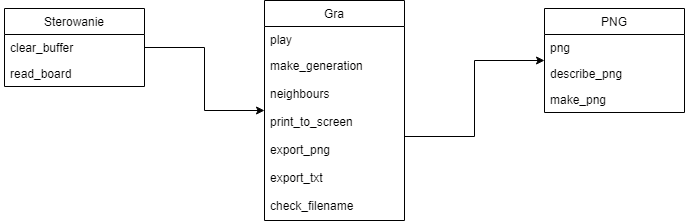
\includegraphics[width=16cm]{diagram.png}
\caption{Diagram modułów}
\label{diagram}
\end{figure}
\section{Testowanie}
Testy zostaną przeprowadzone z wykorzystaniem specjalnie przygotowanych danych przez miniprogramy, które będą wywoływać badane funkcje na danych testowych. Testy będą polegały na sprawdzeniu oczekiwań z wynikami działania miniprogramów. Pliki i dane znaleźć będzie można w folderze \textit{Testy}. Wszystkie komendy do wywołania testów, będą zawarte w pliku Makefile.
\begin{itemize}
    \item Aby przetestować moduł \textit{PNG} przygotujemy plik testowy złożony z 0 i 1~reprezentujących znany nam obraz z czarnych i białych pikseli. Uruchomimy dla tych danych testowych program i sprawdzimy, czy wynik zgadza się oczekiwanym przez nas obrazem.
    \item Aby przetestować moduł \textit{Sterowanie}, podamy różne pliki z danymi, niektóre będą poprawne, a niektóre błędne. Moduł będzie działał poprawnie, jeżeli odrzuci błędne dane i przyjmie poprawne. Przetestujemy tu również \code{clear\_buffer}, wypisując całą planszę razem z buforem i sprawdzimy, czy są w nim same zera.
    \item Moduł \textit{Gra}, będzie wymagał najwięcej testów. Składać się na nie będą:
    \begin{itemize}
        \item testy \code{neighbours} - dla danych które znamy wywołamy funkcję dla konkretnej komórki i sprawdzimy, czy podana wartość zgadza się ze znamymi nam danymi;
        \item testy \code{check\_filename} - wywołamy funkcję dla rożnych danych i sprawdzimy czy odrzuci nazwy zawierające niedozwolone znaki;
        \item testy \code{make\_generation} - wywołamy funkcję dla danych o znanych dla nas wynikach np. szybowiec, lub kwadrat 2 na 2 i z uruchomioną flagą step-by-step będziemy obserwować czy gra przebiega poprawnie.
    \end{itemize}
\end{itemize}
\end{document}





